%
% loesung.tex -- Beispiel-File für die Beschreibung der Loesung
%
% (c) 2020 Severin Weiss, Hochschule Rapperswil
%


\section{Lösung}
\label{laplace:section:Methode nach Talbot}
\rhead{Lösung}
Eine Bedingung um eine passende Kontur zu finden, wurde von Talbot gefunden.
Diese fordert, dass die Singularitäten $s_{j}$ von $F(s)$ bekannt sind, sowie gilt für $F(s)$
\begin{enumerate}
\item
$|F(s)|\rightarrow$ $0$ mit $|s|\rightarrow$ $\infty$ in $Re(s)<\gamma_{0}$
\item
Alle Singularitäten $s_{j} liegen,~~|Im(s_{j})|<K$, wobei der Wert von $K$ bekannt ist.
\end{enumerate}

Die erste Bedingung besagt, dass $F(s)$ für grosse $|s|$ schnell gegen $0$ geht, solange man links von $\gamma_{0}$ ist. Dies hat zur Folge, dass Integrale über Konturen vernachlässigt werden können, wenn sie sich in diesem Gebiet bewegen. Das ist die entscheidende Idee von Talbot und ein entscheidender Vorteil gegenüber der Bromwichkontur, da diese $F(s)$ für grosse $|s|$ nicht genügend schnell gegen $0$ geht. In der Konsequenz verschiebt man die Bromwich-Kontur, wo man nicht vermeiden kann über die ganze imaginäre Achse zu integrieren, sodass man nur noch über einen kleinen Teil integrieren muss. Die beiden Abbildung \ref{laplace:talbot1} und \ref{laplace:talbot2} veranschaulichen die Kontur von Talbot. Darin ist zu erkennen, dass  $|s|$ im Verlaufe der Kontur grösser werden muss. 

\begin{figure}
\centering
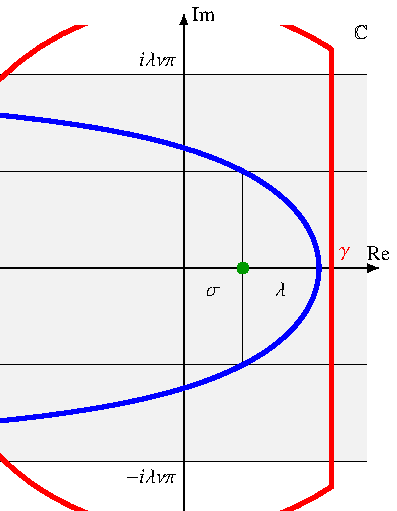
\includegraphics{papers/laplace/images/talbot1.pdf}
\caption{Illustration der Bromwich- und Talbotkontur (breites Band für Singularitäten)
\label{laplace:talbot1}}
\end{figure}

\begin{figure}
\centering
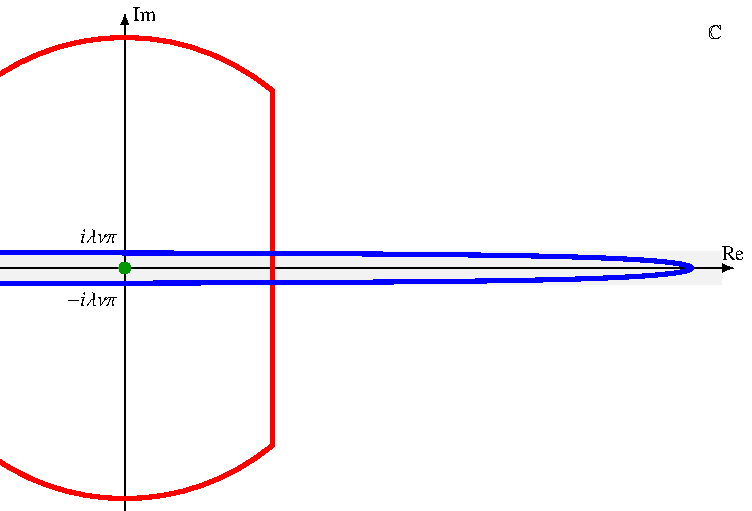
\includegraphics{papers/laplace/images/talbot2.pdf}
\caption{Illustration der Bromwich- und Talbotkontur (schmales Band für Singularitäten)
\label{laplace:talbot2}}
\end{figure}

Die Parameter $\lambda$, $\sigma$ und $\nu$ dienen dazu die
Talbotkontur zu charaktersieren. Eine Erhöhung von $\sigma$ verschiebt
die Kontur nach rechts, während eine Erhöhung von $\nu$ Ausdehnung
in vertikaler Richtung zur Folge hat. Dabei entsteht ein Band der Breite $2i\lambda\mu\pi$, welches symmetrisch zur reellen Achse ist. Das beschriebende Band und dessen Abhängigkeit von den Parametern ist zu erkennen auf den Abbildungen \ref{laplace:talbot1} und \ref{laplace:talbot2}. Die Paramter sollten so gewählt werden, dass die Singularität der Laplacetransformation innerhalb der Talbotkontur, respektive innerhalb des Bandes liegen. 


Die Parametriesierung der Kontur ist gegeben durch
\[
s(z) = \sigma+\lambda s_{\nu}(z),~~ z\in (-2\pi i,~~2\pi i)
\]
wobei
\[
s_{\nu}(z)=\frac{z}{1-e^{-z}}+\frac{z(\nu-1)}{2}
\]

In der Gleichung oben folgt mit $z=2i\theta$ die Parametrisierung
\[
s(\theta) = \sigma+\lambda s_{\nu}(\theta),~~ \theta\in (-\pi ,~~\pi)
\]
wobei
\[
s_{\nu}(\theta)=\theta \cot\theta+i\nu\theta,
\]
und das Riemannsche Inversionsintegral nimmt die Form 
\[
f(t)=\frac{\lambda e^{\sigma}}{2\pi i}\int_{-\pi}^{\pi} e^{-\lambda ts_{\nu}(\theta)}F[\sigma + \lambda s_{\nu}(\theta)]s'_{\nu}(\theta)\,d\theta
\]
an.
wobei
\[
s'_{\nu}(\theta) = i \Biggl\{\nu + \frac{\theta-\cos(\theta)\sin(\theta)}{\sin^{2}(\theta)}  \Biggr\}.
\]
Unter Berücksichtigung der Symmetrie, sowie der Trapezsregel (für detailierte Informationen siehe Kapitel 4) erhält man die Auswertung des Integrals
\[
\tilde{f}(t) = \frac{\lambda e^{\sigma t}}{n}~T_{n}(t)
\]
wobei 
\[
T_{n}(t)
=
{\sum_{j=0}^n}'' e^{\lambda s_{\nu}(\theta_{j})}
F[\sigma + \lambda s_{\nu}(\theta_{j})]
\frac{1}{i} s'_{\nu}(\theta_{j})
\]
\cite{laplace:talbot}

\[
\theta_{j} = j \frac{\pi}{n}.
\]
Die Notation ${\sum_{j=0}^n}''$ besagt, dass der erste und letzte
Term der Summe halbiert werden.
In diesem Falle wird der Term $j=n$ gleich 0 und der $j=0$ Term wird zu
\[
\frac{\nu}{2}e^{\lambda t}F(\sigma + \lambda).
\]


Die obige beschriebene Methode wurde in Python implementiert.

